%-----------------------------------------------------------------------------
% Exercicio 1
\section{Primeiro Exercício: Série de Fourier}

%-----------------------------------------------------------------------------
% 1.a
\subsection{}

\begin{equation}\displaystyle
f(t) = \left\{ 
\begin{array}{l l}
  1, & \quad 0 \le t < 1 \\
  2, & \quad 1 \le t < 2 \\
  0, & \quad 2 \le t < 3 \\
\end{array} \right. \quad \quad f(t+3) = f(t), \forall t \in \mathbb{R}
\end{equation}

\begin{figure}
  \fbox{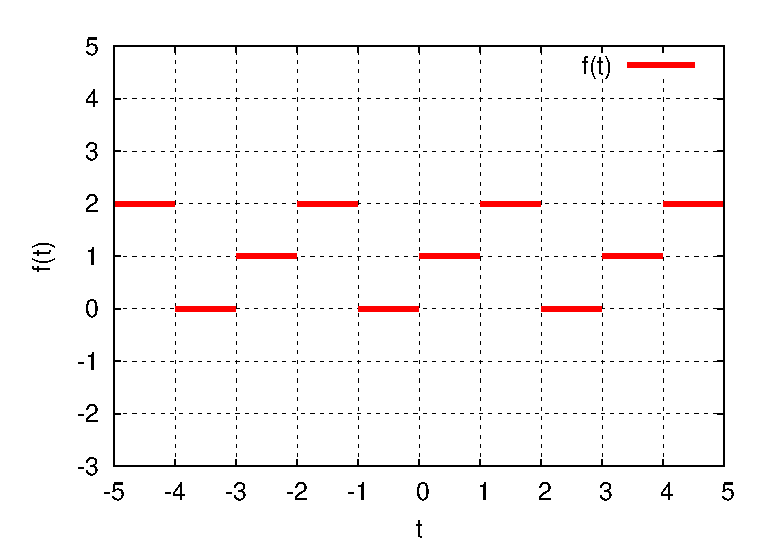
\includegraphics[width=\textwidth]{grafico-1a.eps}}
  \caption{\small{$f(t)$ do exercício \textbf{1.a}.}}
  \label{fig:1a-f}
\end{figure}

$f(t)$ pode ser vista na figura \ref{fig:1a-f}. Notamos pela definição que o período de $f$ é $T = 3$, e que portando sua velocidade angular é $\omega = \frac{2\pi}{3}$ e portanto $\omega_n = \frac{n2\pi}{3}$.

Primeiro, calculamos $F_0$, a primeira parcela da série:

\[\displaystyle
\begin{array}{l c l}
  F_0 & = & \frac{1}{T} \int\limits_0^T \! f(t) e^{-i \omega_0 t} \, dt \quad = \quad \frac{1}{3} \int\limits_0^3 \! f(t) \, dt  \quad = \\
      & = & \frac{1}{3} \left( \int\limits_0^1 \! f(t) \, dt + \int\limits_1^2 \! f(t) \, dt + \int\limits_2^3 \! f(t) \, dt \right) \quad = \\
      & = & \frac{1}{3} \left( 1 + 2 + 0 \right) \quad  = 1
\end{array}
\]

Em seguida, os termos gerais $F_n$ que dependem do harmônico considerado:

\[\displaystyle
\begin{array}{l c l}
  F_n & = & \frac{1}{T} \int\limits_0^T \! f(t) e^{-i \omega_n t} \, dt \quad = \\
      & = & \frac{1}{3} \left( \int\limits_0^1 \! f(t) e^{-i \omega_n t} \, dt + \int\limits_1^2 \! f(t) e^{-i \omega_n t} \, dt + \int\limits_2^3 \! f(t) e^{-i \omega_n t} \, dt \right) \quad = \\
      & = & \frac{1}{3} \left( \int\limits_0^1 \! 1 e^{-i \omega_n t} \, dt + \int\limits_1^2 \! 2 e^{-i \omega_n t} \, dt + \int\limits_2^3 \! 0 e^{-i \omega_n t} \, dt \right) \quad = \\
      & = & \frac{1}{3} \left( \frac{e^{-i \omega_n t}}{-i \omega_n} |_0^1 + 2 \frac{e^{-i \omega_n t}}{-i \omega_n} |_1^2 \right) \quad = \quad \frac{e^{\frac{-2 i n \pi}{3}} -2 e^{\frac{-4 i n \pi}{3}} + 1}{2 i n \pi}
\end{array}
\]

Dessa forma, o $n-$ésimo harmônico fica definido por:

\[\displaystyle
\begin{array}{l c l}
  h_n^f(t) & = & F_n e^{i \omega_n t} + F_{-n} e^{i \omega_{-n} t} \quad = \quad F_n e^{i \omega_n t} + F_n^* e^{-i \omega_{-n} t} \quad = \\
         & = & \left( \frac{e^{\frac{-2 i n \pi}{3}} -2 e^{\frac{-4 i n \pi}{3}} + 1}{i n 2 \pi} \right) e^{\frac{i n 2 \pi t}{3}} + \left( \frac{e^{\frac{2 i n \pi}{3}} -2 e^{\frac{4 i n \pi}{3}} + 1}{-i n 2 \pi} \right) e^{\frac{-i n 2 \pi t}{3}}
\end{array}
\]

E $f(t)$ pode ser escrita como uma soma infinita de todos os harmônicos:

\begin{equation}\displaystyle
  f(t) = 1+ \sum\limits_{n \ge 1} \left[ \left( \frac{e^{\frac{-2 i n \pi}{3}} -2 e^{\frac{-4 i n \pi}{3}} + 1}{i n 2 \pi} \right) e^{\frac{i n 2 \pi t}{3}} + \left( \frac{e^{\frac{2 i n \pi}{3}} -2 e^{\frac{4 i n \pi}{3}} + 1}{-i n 2 \pi} \right) e^{\frac{-i n 2 \pi t}{3}} \right]
  \label{eq:1a}
\end{equation}

O resultado do cálculo de $f(t)$ pela fórmula \eqref{eq:1a} com 100 harmônicos pode ser visto na figura \ref{fig:1a-ffs}.

\begin{figure}
  \fbox{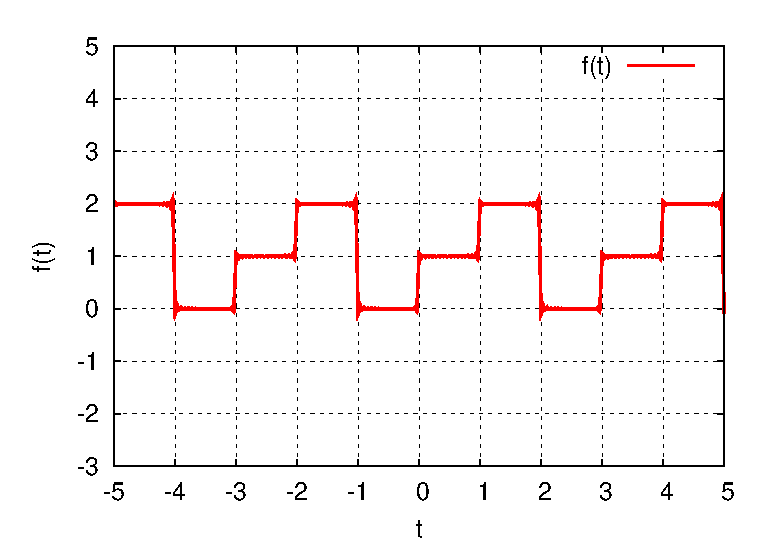
\includegraphics[width=\textwidth]{grafico-1a-transformada.eps}}
  \caption{\small{$f(t)$ do exercício \textbf{1.a} calculada com 100 harmônicos através do cálculo da Série de Fourier.}}
  \label{fig:1a-ffs}
\end{figure}


%-----------------------------------------------------------------------------
% 1.b
\subsection{}

\begin{equation}\displaystyle
g(t) = \left\{ 
\begin{array}{l l}
  sen(\pi t), & \quad 0 \le t < 1 \\
  2 - t, & \quad 1 \le t < 3
\end{array} \right. \quad \quad g(t+3) = g(t), \forall t \in \mathbb{R}
\end{equation}

$g(t)$ pode ser vista na figura \ref{fig:1b-g}. Notamos pela definição que o período de $f$ é $T = 3$, e que portando sua velocidade angular é $\omega = \frac{2\pi}{3}$ e portanto $\omega_n = \frac{n2\pi}{3}$.

\begin{figure}
  \fbox{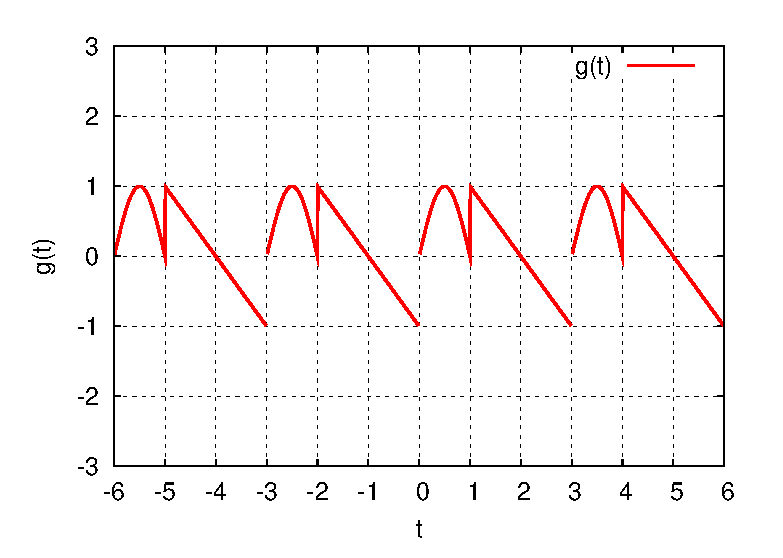
\includegraphics[width=\textwidth]{grafico-1b.eps}}
  \caption{\small{$g(t)$ do exercício \textbf{1.b}.}}
  \label{fig:1b-g}
\end{figure}

Primeiro, calculamos $G_0$, a primeira parcela da série:

\[\displaystyle
\begin{array}{l c l}
  G_0 & = & \frac{1}{T} \int\limits_0^T \! g(t) e^{-i \omega_0 t} \, dt \quad = \quad \frac{1}{3} \int\limits_0^3 \! g(t) \, dt  \quad = \\
      & = & \frac{1}{3} \left( \int\limits_0^1 \! g(t) \, dt + \int\limits_1^3 \! g(t) \, dt  \right) \quad = \quad \frac{1}{3} \left( \int\limits_0^1 \! sen(\pi t) \, dt + \int\limits_1^3 \! (2-t) \, dt \right) \quad  = \\
      & = & \frac{1}{3} \left( \frac{-cos(\pi t)}{\pi} |_0^1 + \left( 2t - \frac{t^2}{2} \right)|_1^3 \right)  = \frac{2}{3 \pi}\\
\end{array}
\]

Em seguida, os termos gerais $G_n$ que dependem do harmônico considerado:

\[\displaystyle
\begin{array}{l c l}
  G_n & = & \frac{1}{T} \int\limits_0^T \! g(t) e^{-i \omega_n t} \, dt \quad = \\
      & = & \frac{1}{3} \left( \int\limits_0^1 \! g(t) e^{-i \omega_n t} \, dt + \int\limits_1^3 \! g(t) e^{-i \omega_n t} \, dt  \right) \quad = \\
      & = & \frac{1}{3} \left( \int\limits_0^1 \! sen(\pi t) e^{-i \omega_n t} \, dt + \int\limits_1^3 \! (2-t) e^{-i \omega_n t} \, dt \right) \quad  = \\
\end{array}
\]

Agora, sabemos que

\[\displaystyle
\begin{array}{l c l}
  \int \! sen(\pi t) e^{-i \omega_n t}\, dt & = & \int \! sen(\pi t) \left( cos(\omega_n t) -i.sen(\omega_n t) \right) \, dt \quad = \\
    & = &  \int \! sen(\pi t)cos(\omega_n t) \, dt -i\int \! sen(\pi t)sen(\omega_n t)
\end{array}
\]

Podemos então calcular as duas integrais separadas, e as contas em anexo mostram que:

\[\displaystyle
\begin{array}{l c l}
  \int\limits_0^1 \! sen(\pi t) e^{-i \omega_n t}\, dt & = & 3 \left( \frac{1-e^{i(\pi-\frac{n2\pi}{3})}}{6\pi - n4\pi} + \frac{1-e^{-i(\pi+\frac{n2\pi}{3})}}{6\pi + n4\pi} \right)
\end{array}
\]

E também que:

\[\displaystyle
\begin{array}{l c l}
  \int\limits_1^3 \! (2-t) e^{-i \omega_n t}\, dt & = & 3 \left( \frac{-e^{-in2\pi}-e^{\frac{-in2\pi}{3})}}{-in2\pi} - 3 \frac{e^{-in2\pi}-e^{\frac{-in2\pi}{3})}}{4 n^2 \pi^2} \right)
\end{array}
\]

Assim, o $n-$ésimo harmônico fica definido por:

\[\displaystyle
\begin{array}{l c l}
  h_n^g(t) & = & G_n e^{i \omega_n t} + G_{-n} e^{i \omega_{-n} t} \quad = \quad G_n e^{i \omega_n t} + G_n^* e^{-i \omega_{-n} t} \quad = \\
         & = & \left[ \frac{1-e^{i(\pi-\frac{n2\pi}{3})}}{6\pi - n4\pi} + \frac{1-e^{-i(\pi+\frac{n2\pi}{3})}}{6\pi + n4\pi} + \frac{-e^{-in2\pi}-e^{\frac{-in2\pi}{3})}}{-in2\pi} - 3 \frac{e^{-in2\pi}-e^{\frac{-in2\pi}{3})}}{4 n^2 \pi^2} \right] e^{\frac{i n 2 \pi t}{3}} \quad + \\
         & + & \left[ \frac{1-e^{-i(\pi-\frac{n2\pi}{3})}}{6\pi - n4\pi} + \frac{1-e^{i(\pi+\frac{n2\pi}{3})}}{6\pi + n4\pi} + \frac{-e^{in2\pi}-e^{\frac{in2\pi}{3})}}{-in2\pi} - 3 \frac{e^{in2\pi}-e^{\frac{in2\pi}{3})}}{4 n^2 \pi^2} \right] e^{\frac{-i n 2 \pi t}{3}}
\end{array}
\]

E $g(t)$ pode ser escrita como uma soma infinita de todos os harmônicos:

\begin{equation}\displaystyle
  g(t) = 1+ \sum\limits_{n \ge 1} h_n(t)
  \label{eq:1b}
\end{equation}

O resultado do cálculo de $g(t)$ pela fórmula \eqref{eq:1b} com 100 harmônicos pode ser visto na figura \ref{fig:1b-gfs}. A princípio podemos desconfiar da inclinação da reta, mas é bom lembrar que foram computados somente 100 harmônicos, e que certamente infinitos harmônicos serão suficientes para conseguir dar a ela a inclinação correta.

\begin{figure}
  \fbox{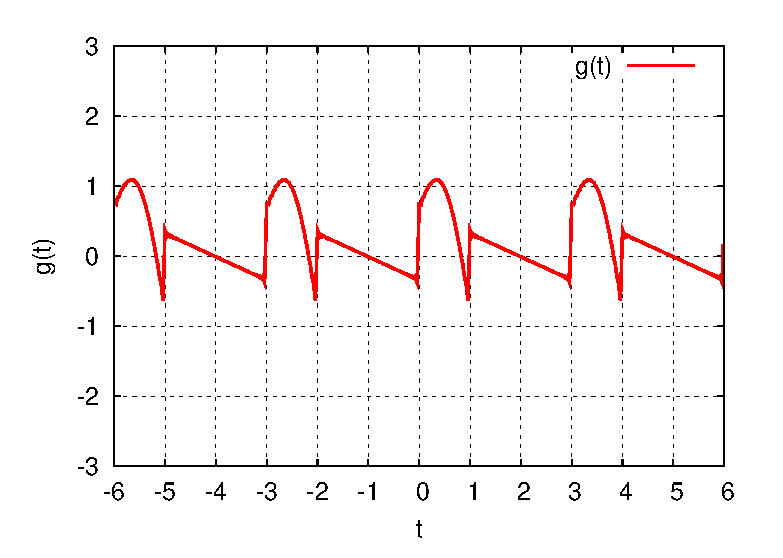
\includegraphics[width=\textwidth]{grafico-1b-transformada.eps}}
  \caption{\small{$g(t)$ do exercício \textbf{1.b} calculada com 100 harmônicos através do cálculo da Série de Fourier.}}
  \label{fig:1b-gfs}
\end{figure}


%-----------------------------------------------------------------------------
% 1.c
\subsection{}

\[\displaystyle
h(t) = 3cos(5t)+2sen(8t) \quad \quad h(t+3) = h(t), \forall t \in \mathbb{R}
\]

\begin{figure}
  \fbox{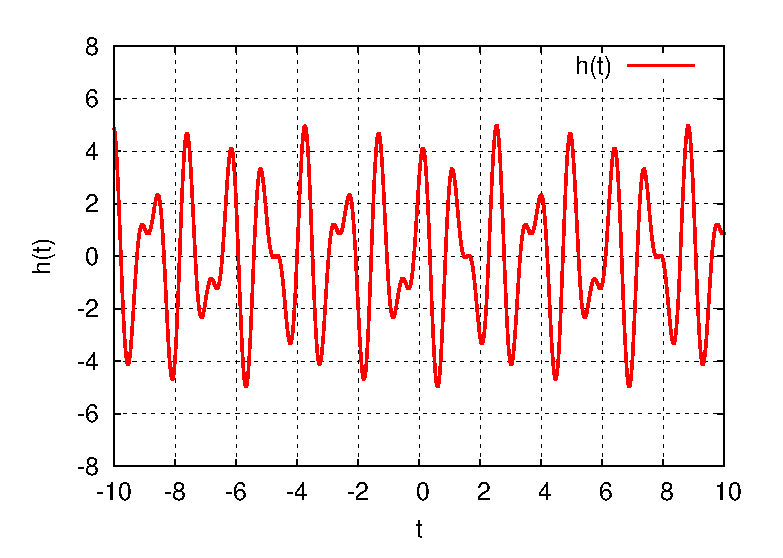
\includegraphics[width=\textwidth]{grafico-1c.eps}}
  \caption{\small{$h(t)$ do exercício \textbf{1.c}.}}
  \label{fig:1c-h}
\end{figure}

$h(t)$ pode ser vista na figura \ref{fig:1c-h}. Podemos encontrar seu período (e velocidade angular) calculando o mínimo múltiplo comum dos períodos em graus dos somandos da expressão:

\[\displaystyle
\begin{array}{l c l}
  \omega_{3cos(5t)} & = & 5 \quad \Rightarrow \quad T_{3cos(5t)} = \frac{2\pi}{5} = 72^o \\
  \omega_{2sen(8t)} & = & 8 \quad \Rightarrow \quad T_{2sen(8t)} = \frac{2\pi}{8} = 45^o \\
  mmc(72,45) & = & 360 \quad \Rightarrow \quad T_h = 2\pi \quad \Rightarrow \quad \omega_n = n
\end{array}
\]

Primeiro, calculamos $H_0$, a primeira parcela da série:

\[\displaystyle
\begin{array}{l c l}
  H_0 & = & \frac{1}{T} \int\limits_0^T \! h(t) e^{-i \omega_0 t} \, dt \quad = \quad \frac{1}{2\pi} \int\limits_0^{2\pi} \! 3cos(5t)+2sen(8t) \, dt  \quad = \\
      & = & \frac{1}{2\pi} \left( 3 \int\limits_0^{2\pi} \! cos(5t) \, dt + 2 \int\limits_0^{2\pi} sen(8t) \, dt \right) \quad = \\
      & = & \frac{1}{2\pi} \left( \frac{3sen(5t)}{5} |_0^{2\pi} + \frac{-2cos(8t)}{8} |_0^{2\pi} \right) \quad = \quad 0
\end{array}
\]

Em seguida, os termos gerais $H_n$ que dependem do harmônico considerado:

\[\displaystyle
\begin{array}{l c l}
  H_n & = & \frac{1}{T} \int\limits_0^T \! h(t) e^{-i \omega_n t} \, dt \quad = \\
      & = & \frac{1}{2\pi} \int\limits_0^{2\pi} \! \left( 3cos(5t)+2sen(8t) \right) e^{-i \omega_n t} \, dt  \quad = \\
      & = & \frac{1}{2\pi} \left( 3 \int\limits_0^{2\pi} \! cos(5t) e^{-i \omega_n t} \, dt + 2 \int\limits_0^{2\pi} sen(8t) e^{-i \omega_n t} \, dt \right) \quad = \\
      & = & \frac{1}{2\pi} \left(3 \int\limits_0^{2\pi} \! cos(5t) cos(nt) \, dt + 2 \int\limits_0^{2\pi} \! sen(8t) cos(nt) \, dt \quad - \right. \\
      & - & \left. 3i \int\limits_0^{2\pi} \! cos(5t)sen(nt) \, dt -2i \int\limits_0^{2\pi} \! sen(8t)sen(nt) \, dt \right) \\
\end{array}
\]

Dos resultados vistos em aula, temos que:

\[\displaystyle
\begin{array}{l c l}

3 \int\limits_0^{2\pi} \! cos(5t)cos(nt) \, dt & = & \left\{
\begin{array}{l l} 
  0, & n \neq 5 \\ 
  3\pi, & n = 5  \\
\end{array} \right. \\

2 \int\limits_0^{2\pi} \! sen(8t)cos(nt) \, dt & = & 0, \, \forall \, n\\
 
-3i \int\limits_0^{2\pi} \! cos(5t)sen(nt) \, dt & = & 0, \, \forall \, n\\
 

-2i \int\limits_0^{2\pi} \! sen(8t)sen(nt) \, dt & = & \left\{
\begin{array}{l l} 
  0, & n \neq 8 \\
  -2i\pi, & n = 8
\end{array} \right.

\end{array}
\]

Assim, o $n-$ésimo harmônico fica definido por:

\[\displaystyle
\begin{array}{l c l}
  h_n^h(t) & = & H_n e^{i \omega_n t} + H_{-n} e^{i \omega_{-n} t} \quad = \quad H_n e^{i \omega_n t} + H_n^* e^{-i \omega_n t}
\end{array}
\]

Como $H_n$ só está definida para $n=5$ e $n=8$, $h(n)$ pode ser escrita como soma de apenas quatro parcelas:

\begin{equation}\displaystyle
\begin{array}{l c l}
  h(t) & = & H_5 e^{i \omega_5 t} + H_5^* e^{-i \omega_5 t} + H_8 e^{i \omega_8 t} + H_8^* e^{-i \omega_8 t} \quad = \\
       & = &  \frac{3}{2} e^{i5t} + \frac{3}{2} e^{-i5t} -i e^{i8t} +i e^{-i8t}
  \label{eq:1c}
\end{array}
\end{equation}

O resultado do cálculo de $h(t)$ pela fórmula \eqref{eq:1c}, com apenas as duas componentes harmônicas, pode ser visto na figura \ref{fig:1c-hfs}.

\begin{figure}
  \fbox{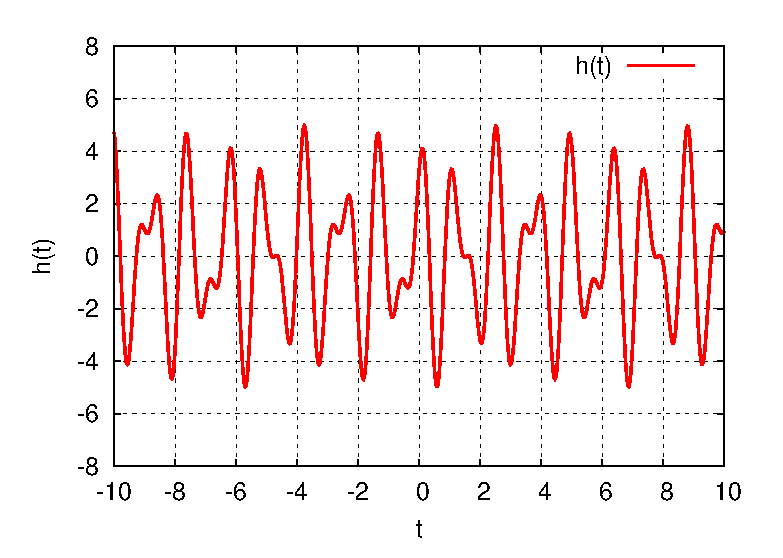
\includegraphics[width=\textwidth]{grafico-1c-transformada.eps}}
  \caption{\small{$h(t)$ do exercício \textbf{1.c} calculada com as duas componentes da transformada de Fourier.}}
  \label{fig:1c-hfs}
\end{figure}


